\documentclass[12pt,a4paper]{article}
\usepackage{fullpage}
\usepackage[top=2cm, bottom=4.5cm, left=2.5cm, right=2.5cm]{geometry}
\usepackage{amsmath,amsthm,amsfonts,amssymb,amscd}
\usepackage{lastpage}
\usepackage{enumitem}
\usepackage{fancyhdr}
\usepackage{mathrsfs}
\usepackage{xcolor}
\usepackage{graphicx}
\usepackage{listings}
\usepackage{hyperref}
\usepackage{tikz}
\usetikzlibrary{shapes,backgrounds}
\usepackage[utf8]{inputenc}
\usepackage[ruled, vlined]{algorithm2e}
% \usepackage{apacite}
\usepackage{csquotes}

% Edit these as appropriate
\newcommand\course{Reinforcement Learning}
\newcommand\NetID{sliu1@uvm.edu}
\newcommand\Author{Sida Liu}
\pagestyle{fancyplain}
\headheight 35pt
\lhead{\NetID\\\Author}
% \chead{\textbf{\Large Assignment \chapternumber }}
\rhead{\course \\ \today}
\lfoot{}
\cfoot{}
\rfoot{\small\thepage}
\headsep 1.5em

\setlength{\parskip}{\baselineskip}%
\setlength{\parindent}{0pt}%

\newenvironment{list_abc}
{ \begin{enumerate}[label=(\alph*)] }
{ \end{enumerate} }

\newenvironment{list_iv}
{ \begin{enumerate}[label=\roman*.] }
{ \end{enumerate} }

\hypersetup{
    colorlinks=true,
    linkcolor=blue,
    filecolor=magenta,      
    urlcolor=cyan,
}

\usepackage{tcolorbox}
\usepackage{booktabs}


\begin{document}

\section*{Technical Plan}

\subsection{Ensemble RL}
In statistics and machine learning, ensemble methods use multiple learning algorithms to obtain better predictive performance than could be obtained from any of the constituent learning algorithms alone. (Wikipedia definition of \emph{Ensemble learning})

\begin{figure}[h]
    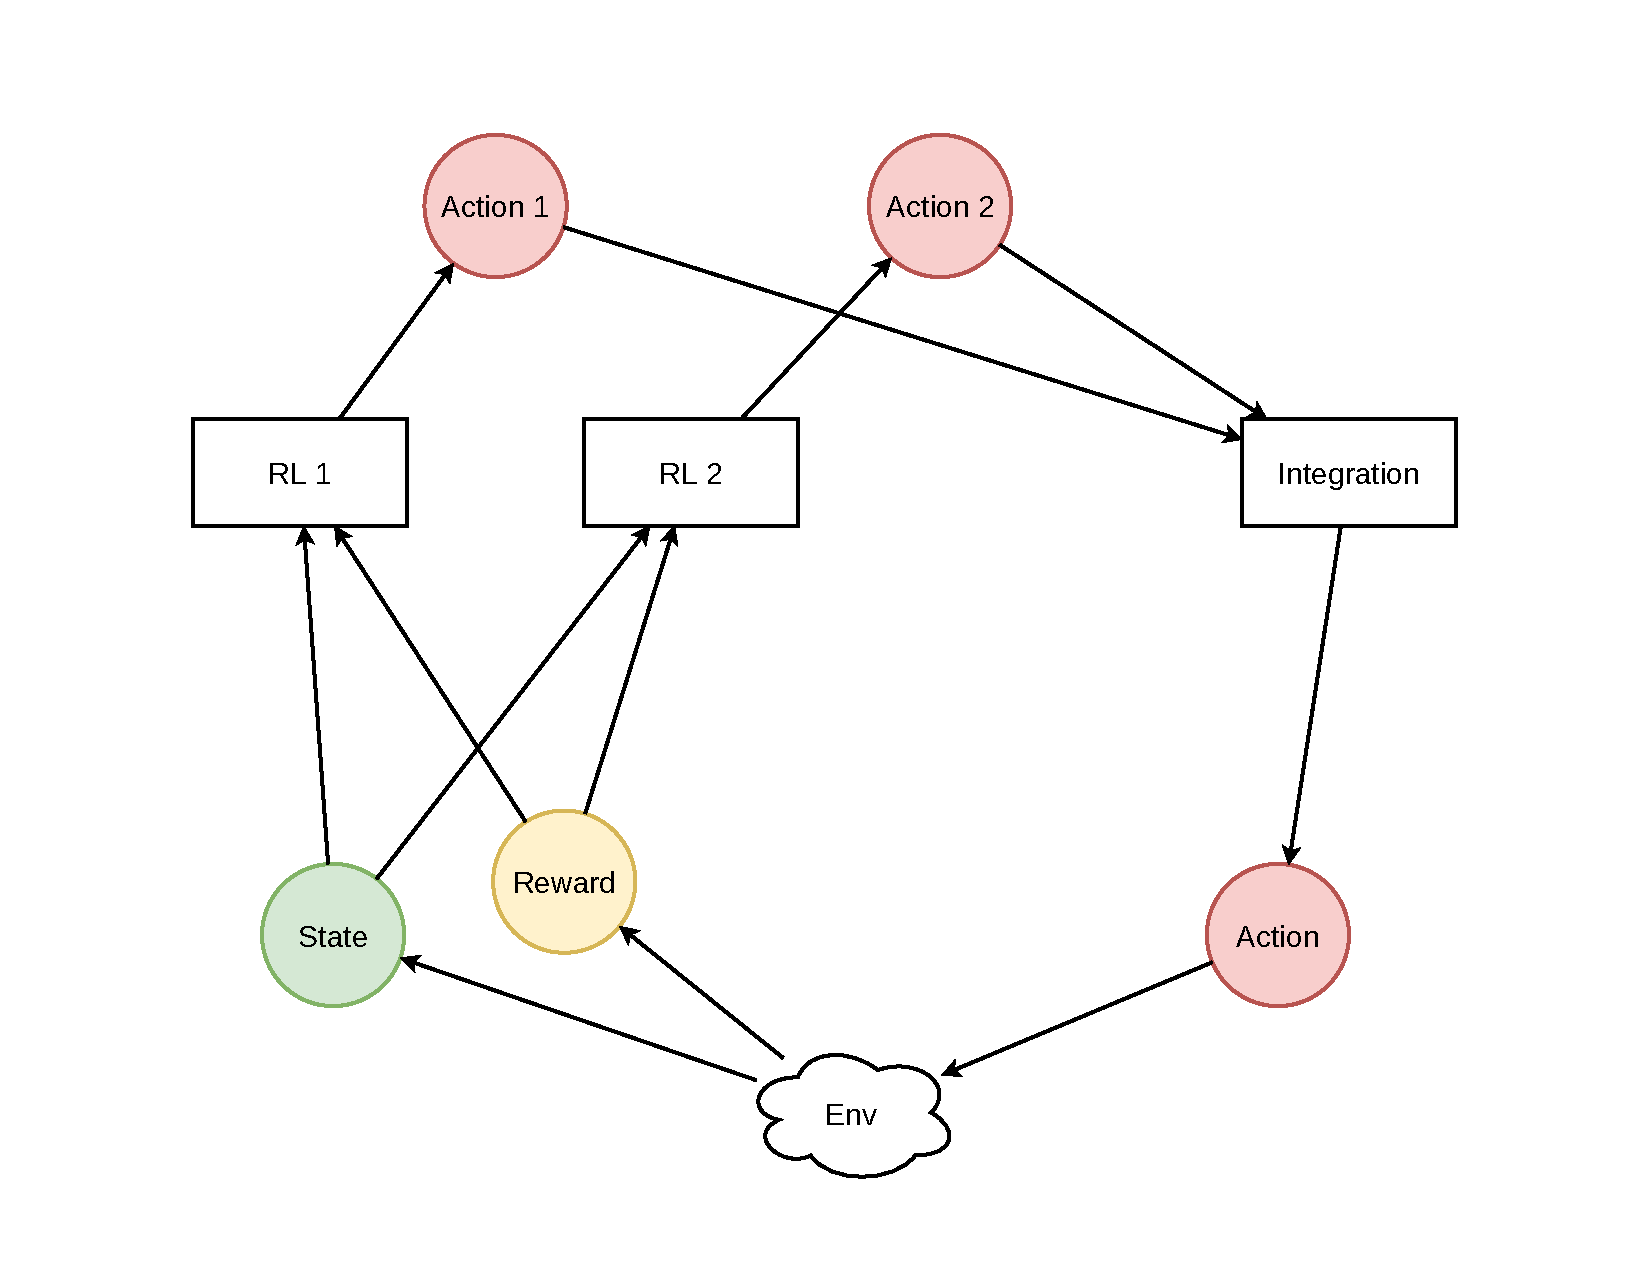
\includegraphics[width=\textwidth]{images/step_1.pdf}
\end{figure}

\newpage
\subsection{Replacing the integration module with an RL}

\begin{figure}[h]
    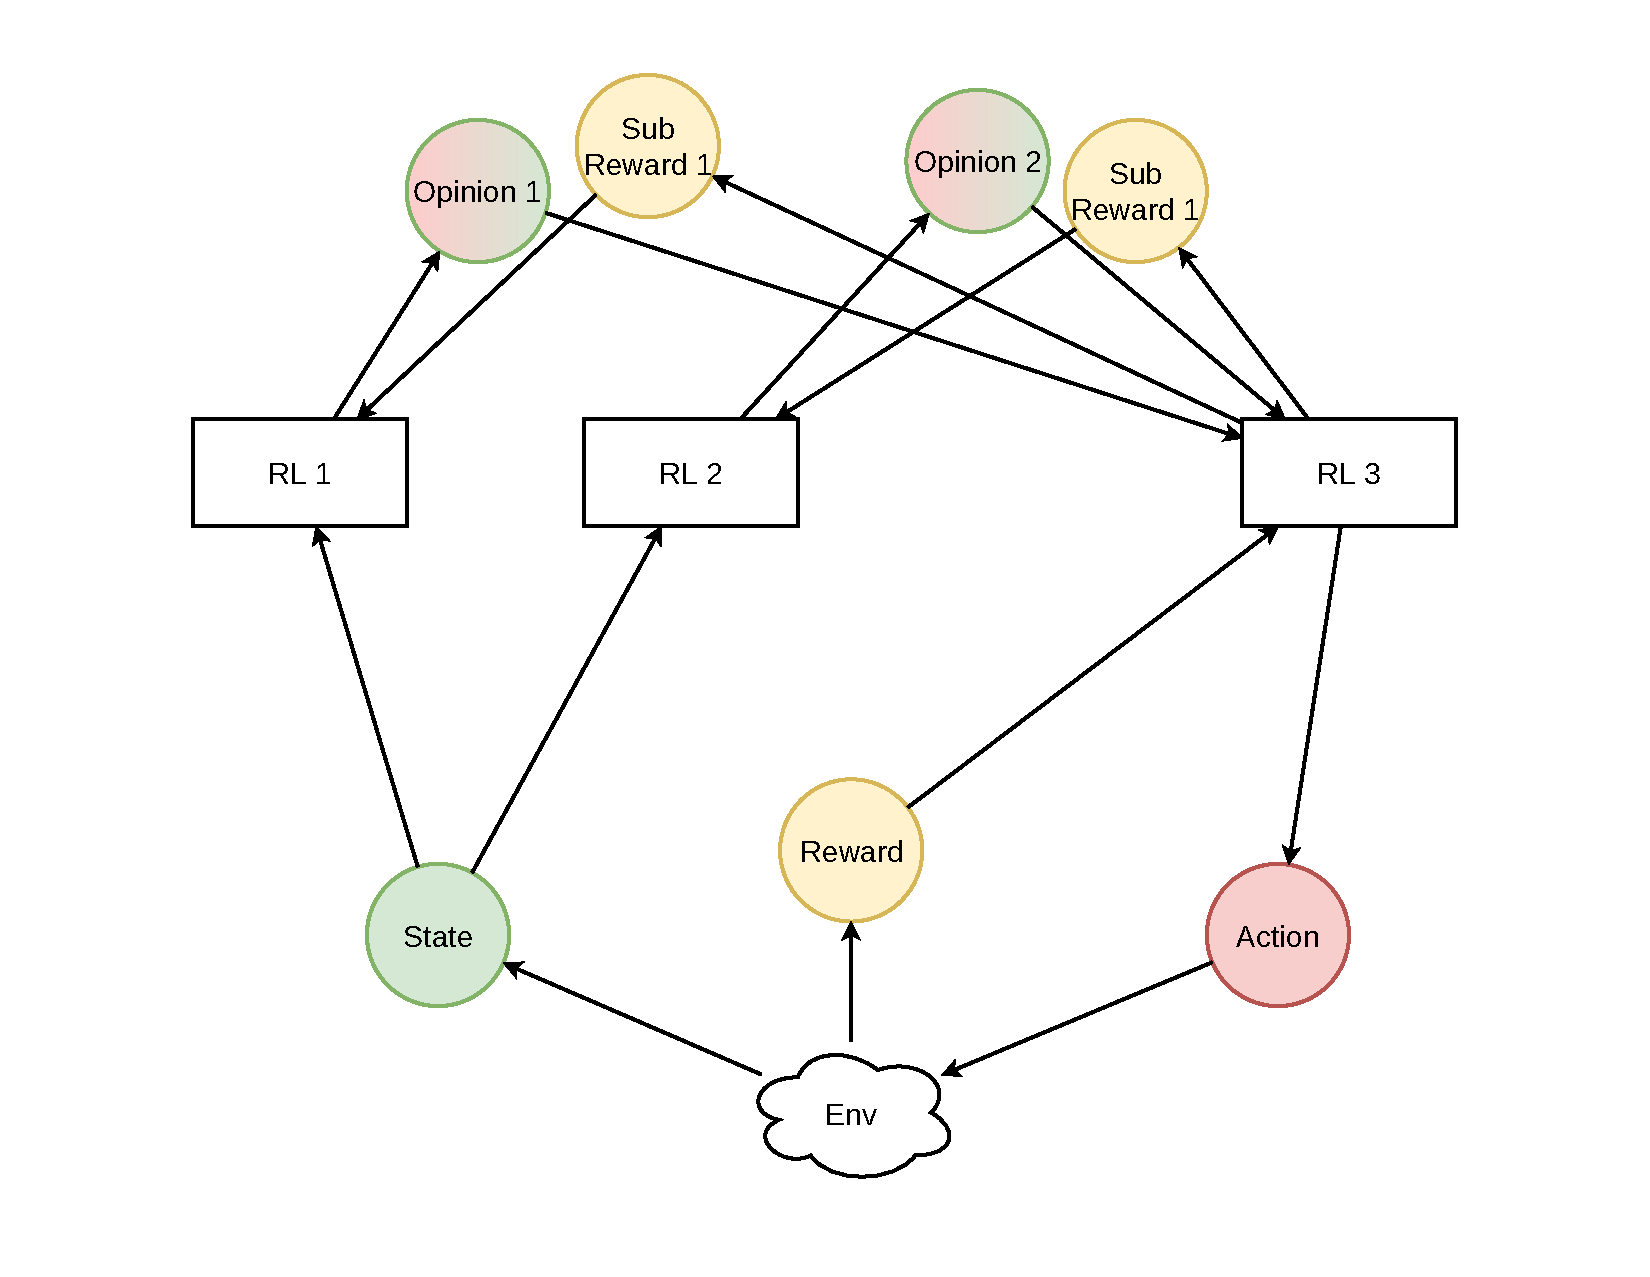
\includegraphics[width=\textwidth]{images/step_2.pdf}
\end{figure}

\newpage
\subsection{High-level RL can pick one specific motory RL to exert action}

\begin{figure}[h]
    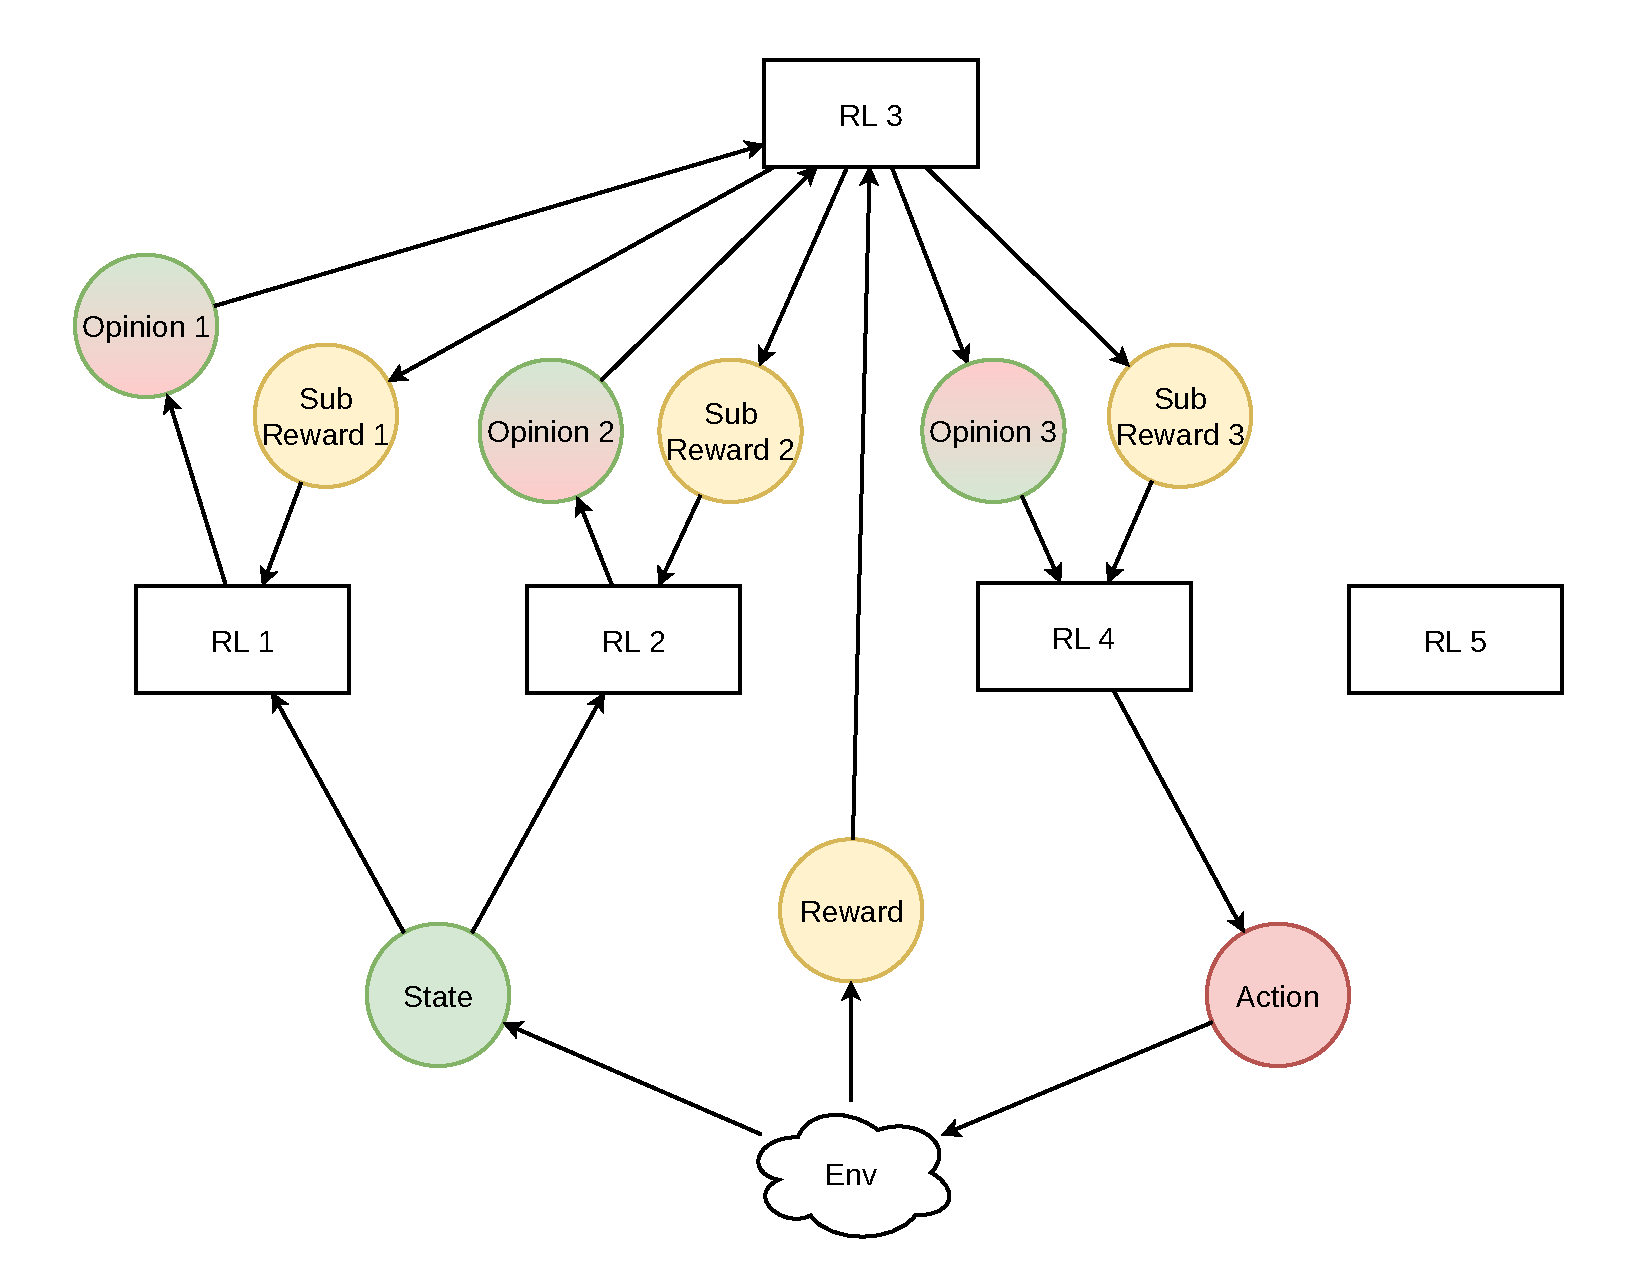
\includegraphics[width=\textwidth]{images/step_3.pdf}
\end{figure}

\end{document}
